% tBPSguide.tex
% v2.1 released November 2014

\documentclass{tBPS2e}

\usepackage{epstopdf}% To incorporate .eps illustrations using PDFLaTeX, etc.
\usepackage{subfigure}% Support for small, `sub' figures and tables
\usepackage{lmodern}
\usepackage{color}
\usepackage[utf8]{inputenc}
\usepackage{float}
\usepackage{lineno}

\theoremstyle{plain}
\newtheorem{theorem}{Theorem}[section]
\newtheorem{lemma}[theorem]{Lemma}
\newtheorem{corollary}[theorem]{Corollary}
\newtheorem{proposition}[theorem]{Proposition}

\theoremstyle{definition}
\newtheorem{definition}{Definition}

\theoremstyle{remark}
\newtheorem{remark}{Remark}

\begin{document}

%\jvol{00} \jnum{00} \jyear{2014} \jmonth{November}

\articletype{Research Article}

\title{\textit{Urban and building multiscale co-simulation: case study implementations on two university campuses}}

\author{Clayton Miller\textsuperscript{a}%
$^{\ast}$\thanks{$^\ast$Corresponding author. Email: miller.clayton@arch.ethz.ch}, 
Daren Thomas\textsuperscript{a},
J\'er\^ome K\"ampf\textsuperscript{b},
and Arno Schlueter\textsuperscript{a}\\
\vspace{6pt}
\textsuperscript{a}{\em Architecture and Building Systems (A/S), Institute of Technology in Architecture (ITA), ETH Z\"urich, Z\"urich, Switzerland};\\
\textsuperscript{b}{\em Solar Energy and Building Physics Laboratory (LESO-PB), Ecole Polytechnique F\'ed\'erale de Lausanne (EPFL), Lausanne, Switzerland}
\received{v0.1 released January 2015}
}

\maketitle

\begin{abstract}
This paper describes the co-simulation process of the building and urban scale models of two campuses of higher education buildings in Switzerland. The campuses are modeled at both the building scale using the EnergyPlus simulation engine and at the urban scale using the CitySim engine. A co-simulation framework is used to execute simulations from both engines concurrently with an exchange of information to leverage the various strengths of each. In the first case study, on-site weather and measured performance data is then compared to the output from two modeling scenarios: building-scale simulation using EnergyPlus and co-simulation of the engines. A partial calibration process is implemented to reconcile the simulations with the measured data a targeted office building on campus. In the second case study, the co-simulation results are compared to the both the CitySim simulation and EnergyPlus engines. The results show that {\color{red}insert results here}. A discussion is included of the challenges encountered with the urban scale calibration and the strengths and weaknesses of the developed process.
\end{abstract}

%Taken out of the abstract: A significant amount of model input information was extracted for the creation of both models from a building information model (BIM) of the campus.

\begin{keywords}
Building-scale simulation, Calibrated energy models, CitySim, Co-simulation, EnergyPlus, Urban-scale simulation 
\end{keywords}


% {\abstractfont\centerline{\bfseries Index to information contained in this guide}\vspace{12pt}
% \hbox to \textwidth{\hsize\textwidth\vbox{\hsize19pc
% \hspace*{-12pt} {1.}    Introduction\\
% \hspace*{7pt} {1.1.}  The \textit{tBPS} document class\\
% \hspace*{7pt} {1.2.}  Submission of \LaTeX\ articles\\
% \hspace*{24pt}        to the journal\\
% {2.}    Using the \textit{tBPS} class file\\
% {3.}    Additional features\\
% \hspace*{10pt}{3.1.}  Title, authors' names, abstract \\
% \hspace*{24pt}        and keywords\\
% \hspace*{10pt}{3.2.}  Additional footnotes to the title \\
% \hspace*{24pt}        or authors' names\\
% \hspace*{10pt}{3.3.}  Lists\\
% {4.}    Some guidelines for using standard\\
% \hspace*{6pt}         features\\
% \hspace*{10pt}{4.1.}   Sections\\
% \hspace*{10pt}{4.2.}   Illustrations (figures)\\
% \hspace*{10pt}{4.3.}   Tables\\
% \hspace*{10pt}{4.4.}   Landscape pages\\
% \hspace*{10pt}{4.5.}   Theorem-like environments\\
% \noindent \hspace*{7pt} {4.6.}   Typesetting mathematics\\
% \hspace*{24pt} {4.6.1.}   Displayed mathematics\\
% \hspace*{24pt} {4.6.2.}   Bold math italic symbols\\
% \hspace*{24pt} {4.6.3.}   Bold Greek\\
% \hspace*{24pt} {4.6.4.}   Upright Greek characters  \\
% \hspace*{50pt}            and the upright partial \\
% \hspace*{50pt}            derivative sign  \\}
% \hspace{-24pt}\vbox{\noindent\hsize19pc
% \hspace*{7pt} {4.7.}   Acknowledgements \\
% \hspace*{7pt} {4.8.}   Funding \\
% \hspace*{7pt} {4.9.}   Notes \\
% \hspace*{7pt} {4.10.}   Supplemental material \\
% \hspace*{7pt} {4.11.}   References \\
% \hspace*{24pt} {4.11.1.}  References cited in the \\
% \hspace*{54pt}            text \\
% \hspace*{24pt} {4.11.2.}   The list of references\\
% \hspace*{7pt} {4.12.}   Appendices \\
% {5.}    Example of a section heading \\*
% \hspace*{7pt}   including \textsc{small caps}, \textit{italic}, \\*
% \hspace*{7pt}   and bold Greek such as ${\bm\kappa}$ \\
% {6.}   {\em tBPS} journal style \\
% \hspace*{10pt}{6.1.}   Hyphens, en rules, em rules \\ \hspace*{27pt}and minus signs\\
% \hspace*{10pt}{6.2.}   References \\
% \hspace*{10pt}{6.3.}   Maths fonts\\
% \noindent   {7.}   Troubleshooting\\
% {8.}   Fixes for coding problems\\
% {9.}   Obtaining the tBPS2e class file\\
% \hspace*{10pt}{9.1}  Via the Taylor \& Francis \\
% \hspace*{24pt}       website \\
% \hspace*{10pt}{9.2}  Via e-mail\\ }}}

\linenumbers

\section{Introduction}

Urban scale building performance simulation is a process that empowers the analysis and optimization of cities. Urban populations are growing around the world at an unprecedented rate. A shift from urban to rural is underway and 2.5 billion people are expected to join urban centers throughout the world \citep{UnitedNations:2014vn}. Expansions of entire districts and even cities is not an uncommon phenomenon, especially in East Asia and Africa. Urban scale modeling is in the midst of a strong focus within the research community with six key areas of practice: technology design, building design, urban climate, systems design, policy assessment, and land use and transportation \citep{Keirstead:2012ct}. The ability to simulate the interaction between large collections of buildings enables the development and testing of optimization and planning scenarios for this new development \citep{Dorer:2013vt}. 

The CitySim simulation engine is an example of such a program designed and optimized for urban-scale simulation. CitySim is an urban performance simulation engine that comprises a Solver module as well as a graphical user interface. It focuses on the energy flows of multiple simplified building models and their interdependent relationship with their urban climate \citep{Robinson:2009tm}. CitySim includes building thermal, urban radiation, occupant behavior, and plant/equipment models integrated as a single simulation engine. CitySim simulates multiple buildings up to city scale using simplified models in order to achieve a good compromise between modeling accuracy, computational overheads and data availability. Each building's thermal behavior is based on an electrical analogy using a two node resistor-capacitor network. The internal lighting, people, and miscellaneous loads are modeled using a simplified occupancy-based approximation. The heating, ventilation, and air-conditioning (HVAC) systems are modeled using a single equation that approximates the total mass flow rate required to meet the sensible and latent loads of each building as a whole. Each of these simplifying approximations empowers the urban-scale simulation to have reasonable execution times with respect to the number of buildings being simulated.

Building performance simulation is a mature domain of research relative to urban scale efforts. The use of whole building simulation engines originated in the 1960s with the US government's development of the BLAST and DOE-2 hourly energy simulation programs \citep{Lawrie:2001vf}. In 1996, development on a new simulation engine, EnergyPlus, began in order to combine the advantages of previous efforts in a single, modular program. EnergyPlus, as a result, has become a popular choice in detailed whole-building performance simulation due to the breadth of mechanical, renewable, and electrical systems that can be modeled. EnergyPlus specifically excels in its ability to model unique mechanical system types such as decoupled centralized cooling \citep{Miller:2010wa} and low exergy heating and cooling systems \citep{barbara:2015tz}. Additionally, EnergyPlus is designed to provide a high resolution in which internal loads and natural ventilation technologies can be modeled in detail at the building level.  

Both building and urban-scale simulation domains have rightfully chosen boundary conditions that reflect their key goals while seeking to minimize the input parameters necessary and run-times of the engines themselves. This focus results in certain deficiencies with respect to modeling various phenomenon. For example, urban scale simulation highly simplifies the building systems and internal load models, thus making retrofit analysis at the systems level difficult. And whole building simulation neglects many of the various contextual consideration of the urban environment such as long wave radiation exchange with adjacent surfaces and localized urban weather effects.

In order to address the deficiencies of the individual engines, the current effort described seeks to couple building and urban scale simulation. The research in this paper is part of an larger coupling effort in which various engines are connected and co-simulated to create a more comprehensive analysis of the urban scale \citep{Dorer:2013vt}. The target is the computational interface between the building energy model, using EnergyPlus, and the urban energy model using CitySim. An overview of the larger scope is shown in Figure \ref{fig:UMEM} and the context of the coupling task is shown as the interface between the City Energy Simulation (CES) model and the Building Energy Simulation (BES) model.

The coupling and co-simulation process is implemented on two case studies in Switzerland. The first case study is the ETH Z\"urich Hoenggerberg campus in Z\"urich, Switzerland. The campus was modeled in the CitySim simulation engine and co-simulated using work-flow automation. The target of this case study is to evaluate the differences between the coupled and uncoupled EnergyPlus simulation results with a target on the use of these models for building retrofit analysis. This scenario includes the use of measured data for heating and cooling within their respective seasons to compare to the simulation results. The second case study is the EPFL campus in Lausanne, Switzerland. The objective of this scenario is to evaluate the differences between coupled and uncoupled versions of the CitySim simulation engine. 

\begin{figure}
\centering
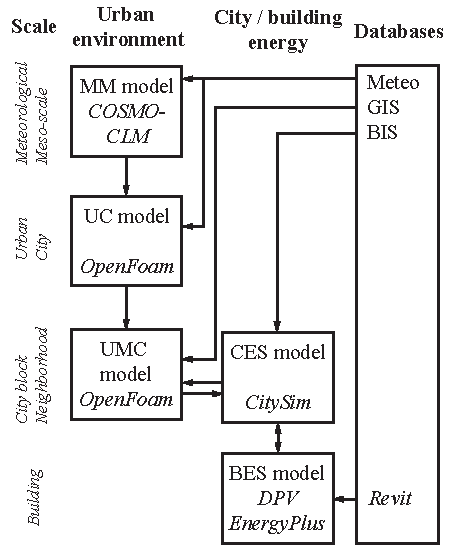
\includegraphics[scale=0.7]{figures/UMEM_overview_new}
\caption{EnergyPlus and CitySim coupling are part of the wider context. Each block in the diagram represents an environment, with the tool/engine name in italics (adapted from \citep{Dorer:2013vt})}
\label{fig:UMEM}
\end{figure}

This paper describes the achievement of several objectives:
\begin{enumerate}
  \item Automation of the process of simultaneous meta-data extraction from a building information model (BIM) for the creation of both building and urban-scale performance models for a real-world campus of buildings
  \item Co-simulate the urban and building scale models through concurrent information exchange
  \item Implement a simplified calibration procedure based on reconciling the co-simulation output results for a selected subset of buildings that have adequate measured energy performance data from the campus energy information system (EIS) 
\end{enumerate}

The first two objectives have been demonstrated in a simplified context in previous literature \citep{thomas2014multiscale,Miller:2015vk}. The novelty of the current publication is an extension to this research through the modelling and co-simulation of real-world case studies. The third objective is completely novel in that no previous study has compared the results of a building and urban-scale co-simulation procedure to measured data from a real-world campus. 

\subsection{Previous multi-scale coupling studies}
Previous attempts of information exchange have been implemented between simulation engines at various scales. Much of the initial co-simulation work is at the subsystem and building-scales. Previous studies have analyzed strong and loose coupling of engines at this scale \citep{Trcka:2010cr,Wetter:2011kh}. Coupling of building-scale simulation with urban-scale computational fluid dynamics (CFD) is attempted for modelling natural ventilation \citep{Zhang:2013vx} and to improve energy prediction \citep{Bouyer:2011eha}. EnergyPlus has been coupled with ENVI-met, a micro-climate computational fluid dynamics (CFD) program \citep{Yang:2012cr}. It was also coupled with simplified lumped parameter models in order to facilitate comparison with measured sensor data \citep{Martin:2015fj}. EnergyPlus and the TEP Urban Canopy Model program were coupled in order to quantify the influences of urban localized weather effects on whole building simulation \citep{Bueno:2011hi}. 
% \subsection{Urban scale performance simulation}

\section{Methodology}\label{Methodology}
% A significant amount of the following methodology is developed in previous literature and is reiterated in this section in order to set the context for Section \ref{Implementation}. The previous published research is clearly outlined at the beginning of each subsection.

\subsection{Coupling process}
The coupling process of a simplified single zone model and contextual surrounding buildings is outlined in a previous study \citep{thomas2014multiscale}. This study forms the basis for the methodology in the current effort. This process utilizes the Design Performance Viewer (DPV) and associated work flow. The DPV is a tool written to extract and simulate an EnergyPlus input data file (IDF) from an Autodesk\textsuperscript{TM} Revit\textsuperscript{TM} BIM \citep{Schlueter2009}. The main philosophy behind the tool is rapid simulation of the building information model from the earliest design possible and can be used throughout the life-cycle of the building including retrofit analysis \citep{Miller:2014tu}. This process is achieved by augmenting the information in the BIM with default values and abstracting information not relevant for energy simulation. The tool already has a simplified notion of surrounding buildings, which are modeled in the BIM as simple mass objects without further information and are exported as shading surfaces to EnergyPlus. This functionality is used for creating the CitySim mass scene and leads to a crude model of the urban context of the building. The existing DPV philosophy of allowing the designer to iterate rapidly on early design decisions based on feedback about the performance of the design remains. This approach includes streamlining the process where running a simulation requires no effort from the designer due to automatic creation of input files, execution and analysis of the results.

The coupling process of EnergyPlus and CitySim is shown in Figure \ref{fig:OverallWorkflowProcess}. First, the DPV is used to extract an EnergyPlus simulation model from the BIM. The DPV utilizes the Revit API to extract geometrical information about the building and the physical properties of walls, windows, doors, roofs and floors. This information is encoded in the BIM model as wall types, roof types,
floor types as well as window and door families. Wherever possible, the tool uses the layering and materials of the construction types, enhancing them with physical attributes relevant to EnergyPlus. Where not defined, it assumes default values.

\begin{figure}[H]
\centering
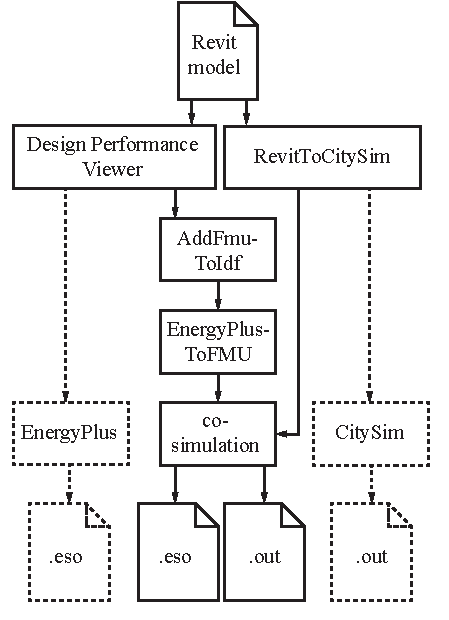
\includegraphics[scale=0.7]{figures/UMEM_Workflow}
\caption{Overview diagram of the coupling process including tools and outputs (adapted from \cite{thomas2014multiscale})}
\label{fig:OverallWorkflowProcess}
\end{figure}

Next, geometry is created to be used in both the CitySim and EnergyPlus models as buildings and surfaces surrounding the building targeted in the IDF. This feature of the DPV is used for including shading surfaces in the EnergyPlus simulation model: it uses so-called \emph{mass objects} in the BIM model as surrounding buildings. The DPV model views these buildings as a series of shading surfaces. A transformation is added on the DPV model that produces an input file for the CitySim solver. This file uses an XML format describing the buildings in a scene for simulation, including their construction types, geometry and systems for heating and cooling. The main BIM is extracted to the CitySim scene as one of the buildings to be simulated, with the properties of the construction types matching those in the DPV model. The glazing ratio is calculated based on the window and wall areas of the DPV model. Shading surfaces are grouped into buildings based on the mass object they were extracted from. These neighboring buildings use default construction properties for walls and roofs and we assign them a default glazing ratio. These defaults can be overridden by custom properties applied to the mass objects in the BIM much in the same way as the model elements of the main building are enriched with DPV information. 

As of version 8.1.0, EnergyPlus supports exporting a simulation model as a Functional Mock-up Unit (FMU) \citep{Nouidui:2014hq}. This feature introduces new IDF objects to specify the interface such an FMU exposes. These objects define which output variables are exported by the FMU and which variables are imported. The FMU export functionality is closely linked to the Energy Management System (EMS) of EnergyPlus. Co-simulation exchange variables either mimic an EnergyPlus schedule, an EMS variable or drive an EMS actuator. It was determined that in order to export an output variable using the FMU export functionality, the variable itself must also be output with an IDF object of type \emph{Output:Variable} or \emph{EnergyManagementSystem:OutputVariable} in the IDF file as well. Since the model used by CitySim to simulate a building is more abstract than the model used by EnergyPlus, the EMS is used to aggregate certain values. CitySim does not model windows separately, therefore a weighted average of window and wall surface temperatures is calculated with EMS subroutines.

\begin{figure}[H]
\centering
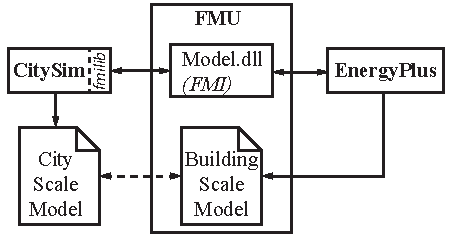
\includegraphics[scale=0.7]{figures/UMEM_FMU_Overview}
\caption{Simulation information exchange between CitySim and EnergyPlus using FMI (adapted from \cite{thomas2014multiscale})}
\label{fig:FMUOverview}
\end{figure}

% The process of augmenting the IDF file is automated with the EMS subroutines and FMU export objects. The script \emph{addfmutoidf.py}, written in the Python programming language, uses the \emph{parseidf} module to read in the IDF file and add the new IDF objects based on those found in the model.  This script reads in the list of surfaces defined in the IDF file and produces EMS scripts to aggregate and output the surface temperatures of the wall and the windows as well as any other output objects necessary.

The FMU creation process is the basis for coupling the two models at each timestep in the simulation. Figure \ref{fig:FMUOverview} illustrates this process from both the EnergyPlus and CitySim perspective. The augmented IDF file is fed to the \emph{EnergyPlusToFMI} script \citep{Nouidui:2014bo}. Once configured, this script produces an FMU file based on the augmented IDF file and the weather file to be used as well as a DLL file implementing the Functional Mock-up Interface that can load the IDF file, locate EnergyPlus and run the simulation. Table \ref{FMUimports} and \ref{FMUexports} outline the variables exchanged between EnergyPlus and CitySim through the FMI. 

% We used the \emph{fmilib} library from the JModelica project to test the FMU produced \citep{Anonymous:ZZTfF80-}. We altered one of the sample programs (\emph{fmi\_import\_cs\_test.c}) to load the FMU, run it and print out the values exported from EnergyPlus. This code was then used as a guide to extending the CitySim solver to load FMUs for co-simulation.

\subsection{Coupled variables}

On an hourly basis, CitySim performs a heating and cooling needs prediction step. The temperature determination step for the main building is replaced with the results of the EnergyPlus timestep as obtained through FMI library. The FMI library is used to send climatic and occupational data from CitySim to EnergyPlus (see Table \ref{FMUimports}), and to receive data from EnergyPlus that are further used within CitySim for the next time steps (see Table \ref{FMUimports}).

\begin{table}[H]
\tbl{Values imported by EnergyPlus from CitySim by the FMU}
{\begin{tabular}[l]{@{}lcc}\toprule
  \bf{Object (ep\_id)} &  \bf{Variable Name} & \bf{Description} \\
\colrule
  Outdoor & Outdoor Drybulb & The outdoor dry-bulb temperature in $^{\circ}\mathrm{C}$ \\
 & Outdoor Dewpoint & The outdoor dewpoint temperature in $^{\circ}\mathrm{C}$ \\
 & Outdoor Relative Humidity & The outdoor relative humidity expressed in percent. \\
 & Diffuse Solar & Diffuse horizontal irradiance in W/m$^2$ \\
 & Direct Solar & Beam normal irradiance in W/m$^2$ \\
 & Wind Speed & The outdoor wind speed in m/s \\
 & Wind Direction & The wind direction in degrees\\&&  (N=0, E=90, S=180, W=270) \\
 \hline
 Long Wave Radiation & Environmental Radiant Temp. & Calculated $T_{env}$ from the sky,\\&& ground, and surrounding surfaces \\
 & Environmental Radiant Heat & Calculated $h_{env}$ from the sky,\\&& ground, and surrounding surfaces \\
 & Gain Coefficient \\
 \hline
Zone & Occupation & Fraction of the maximum occupation\\&& (0.0-1.0) overrides the EnergyPlus occupation schedule\\&&  with the CitySim stochastic schedule. \\
\botrule
\end{tabular}}
\label{FMUimports}
\end{table}

\begin{table}[H]
\tbl{Values exported by EnergyPlus to CitySim by the FMU}
{\begin{tabular}[l]{@{}lcc}\toprule
  \bf{Object (ep\_id)} &  \bf{Variable Name} & \bf{Description} \\
\colrule
Wall, Roof & Outside Surface Temperature & The temperature on the outside of the surface in $^{\circ}\mathrm{C}$ \\    
    \hline
Wall & Average Outside Surface Temperature & The (weighted) average temperature of \\
& & the surface on the outside in $^{\circ}\mathrm{C}$. \\
    \hline
Zone & Total Heating Energy & The heating energy in Joules used in this timestep. \\
& Total Cooling Energy & The cooling energy in Joules used in this timestep. \\
& Zone Mean Air Temperature & The mean air temperature in the zone in $^{\circ}\mathrm{C}$ \\
& Ventilation Volume Flow Rate & The flow rate in $\mathrm{m}^3/\mathrm{s}$ (standard density) \\
\botrule
\end{tabular}}
\label{FMUexports}
\end{table}

\subsection{Long wave radiation exchange}

Long wave radiation exchange in the urban scale environment is also coupled in the co-simulation process. However, it requires the development of a set of approximations to reduce the number of coupled variables between the engines and to account for differences in the methods by which each engine calculates this metric. A detailed description of Long Wave Radiation (LWR) variable exchange and approximation is found in a previously published study \citep{Miller:2015vk} on a simplified theoretical case. 

In EnergyPlus, LWR exchange for a surface is calculated through the summation of radiation gain from the ground, sky, and air as seen in Equation \ref{EPlus_LWR_Ext} and Figure \ref{combinedLWR}a \citep{doe2010energyplus}. The radiant heat transfer coefficient for each of these environmental variables is calculated according to Equation \ref{EPlus_h} with $\sigma$ as the Stefan-Boltzmann constant and $\epsilon$ as the emissivity. A major assumption of this approach is that the modeled building's surfaces and those of adjacent buildings are at a uniform temperature and the LWR radiation exchange is negligible; a situation that is an oversimplification in an urban
scale domain \citep{Evins:2014cf}.
\begin{equation} \label{EPlus_LWR_Ext} 
Q_{LWR,EnergyPlus} = h_{r,grd}(T_{surf}-T_{grd}) + h_{r,sky}(T_{surf}-T_{sky}) + h_{r,air}(T_{surf}-T_{air})
\end{equation}
\begin{equation} \label{EPlus_h} 
h_{r,variable} = \frac{\epsilon\sigma(T^{4}_{surf}-T^{4}_{variable})}{T_{surf}-T_{variable}}
\end{equation}

In comparison, CitySim calculates LWR exchange by calculating an aggregated equivalent temperature, $T_{env}$, and radiative heat transfer coefficient, $h_{r,env}$, from surrounding urban surfaces in addition to ground, sky, and air \citep{Robinson:2009tm}. The calculation for $T_{env}$ is expressed in Equation \ref{CitySim_Tenv} with the $F$ values being view factors of the surrounding environment including adjacent surfaces $i=1..n$. $h_{r,env}$ is based on a first order Talyor development of the numerator of Equation \ref{EPlus_h} around $(T_{surf}+T_{variable})/2$ and therefore $Q_{LWR,CitySim}$ is calculated using Equation \ref{CitySim_LWR_Ext}.
\begin{equation} \label{CitySim_Tenv} 
\sigma T_{env}^4 = \sigma F_{sky}T_{sky}^4 +\sigma F_{grd}T_{grd}^4 + \sum_{i=1}^{n} \epsilon_i \sigma F_{i}T_{i}^4
\end{equation}
\begin{equation} \label{CitySim_LWR_Ext} 
Q_{LWR,CitySim} = h_{r,env}(T_{surf}-T_{env})
\end{equation}

In the coupled simulation, EnergyPlus uses the CitySim supplied equivalent $h_{r,env}$ and $T_{env}$ to calculate weighted $h_{r,sky}$, $h_{r,grd}$, and $h_{r,air}$ values using the view factors and the sky-to-air split ratio. Figure \ref{combinedLWR} illustrates the schematic differences between the solo and coupled simulations on a theoretical example of a target building with two adjacent buildings with surfaces available for radiation exchange.

\begin{figure}[H]
  \centering
  \includegraphics[width=1.0\textwidth]{figures/LWRCalc_Combined_V3}
  \caption{Comparison of the LWR components between a) Solo EnergyPlus and b) Coupled CitySim/EnergyPlus configuration (adapted from \citep{Miller:2015vk})
  \label{combinedLWR}}
\end{figure}


\subsection{Simplified calibration}
In the first case study, one aspect of this analysis is the comparison of actual measured performance of a buildings on campus with the simulation results of the co-simulation. A simplified calibration procedure is adapted from previous research to compare the measured heating and cooling data available on campus with various simulation scenarios \citep{Samuelson:2015jg}. This calibration procedure was utilized in the performance reconciliation of 18 buildings that were built according to the LEED Canada protocol and were under review of actualized performance. This protocol is unique in its analysis process to uncover design model deficiencies in a step-wise manner, utilizing the most easily accessible knowledge first and working towards equilibrium between measured and simulated. An appropriate balance between effort of implementation and value generated through the calibration process. 

% The following steps are the general procedure applied to the targeted buildings:

% \begin{enumerate}
%   \item Using the local weather conditions for the simulation period
%   \item Update simulation based on custom lighting schedules and power densities extracted from the measured data
%   \item Update simulation based on custom plug load schedules and power densities extracted from the measured data
%   \item Account for \emph{unregulated} building loads such as experimental equipment and process loads
% \end{enumerate}
 
\section{Implementation}\label{Implementation}
The co-simulation process is implemented on two case studies in Switzerland. The first is the ETH Z\"urich Hoenggerberg campus in Z\"urich, Switzerland. The focus of this case study is to compare the impact of the information exchange through co-simulation within the EnergyPlus engine. The intent on this campus was to develop techniques for retrofit analysis using EnergyPlus. The targeted building on this campus is the HPI Building. Raw measured data is available for many of the buildings on campus, thus a simplified calibration procedure is used to reconcile the simulation results.\\

The second case study is the EPFL campus in Lausanne, Switzerland. The targeted building in this case was the Quartier Nord complex. The focus of this study was to compare the output results of both CitySim and EnergyPlus. Reliable measured data for calibration is not currently available for this building.

\subsection{Campus case study 1: ETHZ Hoenggerberg Campus}
% {\color{red}This section will describe the ETH Hoenggerberg case study}
%The simulation and calibration process is implemented on a campus case study located in Z\"urich, Switzerland. 
The ETH Z\"urich Hoenggerberg campus includes 32 higher education buildings with spaces allocated to laboratories, office space, lecture halls, cafeterias, data centers and other types of similar spaces. The campus has a centralized energy management system (EMS) that contains 807 energy and water measurement points from heating, cooling, electricity, city gas, domestic hot water, grey water, and general water consumption. 

%Figure \ref{fig:pointgraph} illustrates the breakdown of these measurement system data points amongst the campus buildings.

% \begin{figure}
% \centering
% 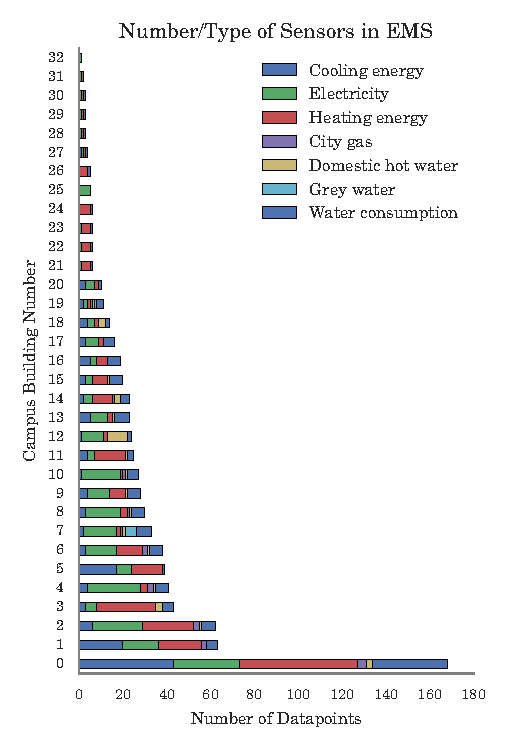
\includegraphics[scale=0.7]{figures/pointbreakdown_anon}
% \caption{Available performance measurement points}
% \label{fig:pointgraph}
% \end{figure}

The focus of the co-simulation process is that the performance of a targeted building is evaluated through solo and coupled methods. The HPI building on campus was chosen in this case study due to amount and quality of measured data available from the EMS for this building. The HPI building is indicated on a campus map shown in Figure \ref{fig:campusmap} and is shaded red.

% The coupling process outlined is applicable with regards to a targeted building that is surrounded by an adjacent array of buildings. 
% {\color{red}Insert the campus map illustrating the targeted buildings.}

\begin{figure}[H]
\centering
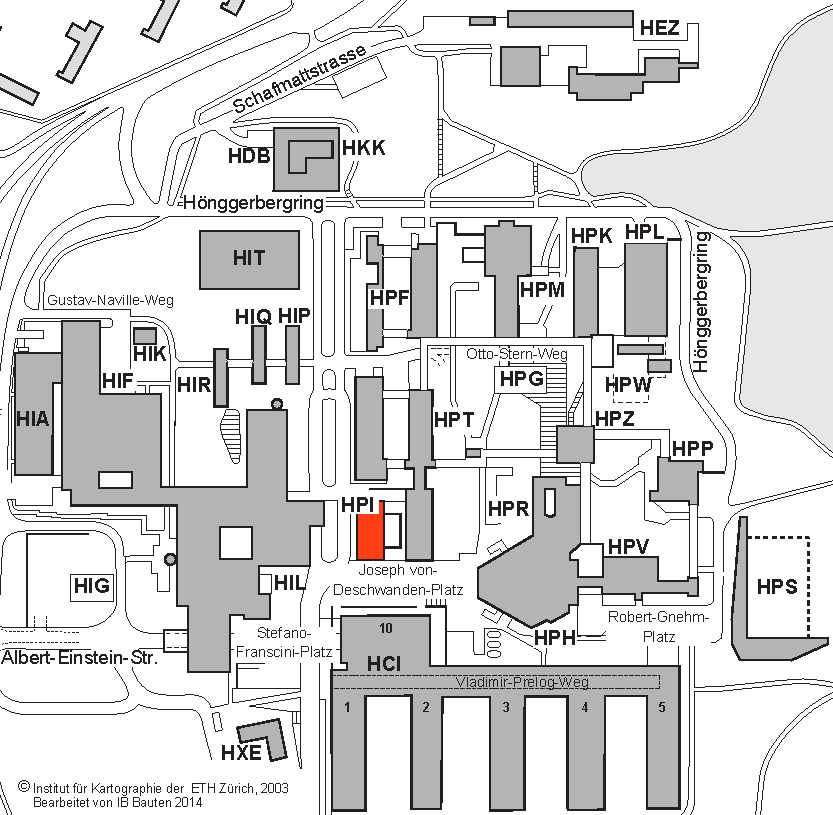
\includegraphics[scale=0.5]{figures/ETH_Hoenngerbergcamp_targetedbuildings_HPI}
\caption{ETH Hoenggerberg campus map with the HPI building shaded red}
\label{fig:campusmap}
\end{figure}

\subsection{Model development}
In order to perform a co-simulation of the targeted buildings, initially a CitySim model of the campus is developed. Through the workflow automation process, this geometry was converted into an EnergyPlus input file as seen in Figure \ref{fig:HPIcampus}. 
% An existing EnergyPlus model is used for the HPZ building and simplified single-zone EnergyPlus models are extracted from the CitySim geometry for the other three targeted buildings.

\begin{figure}[H]
\centering
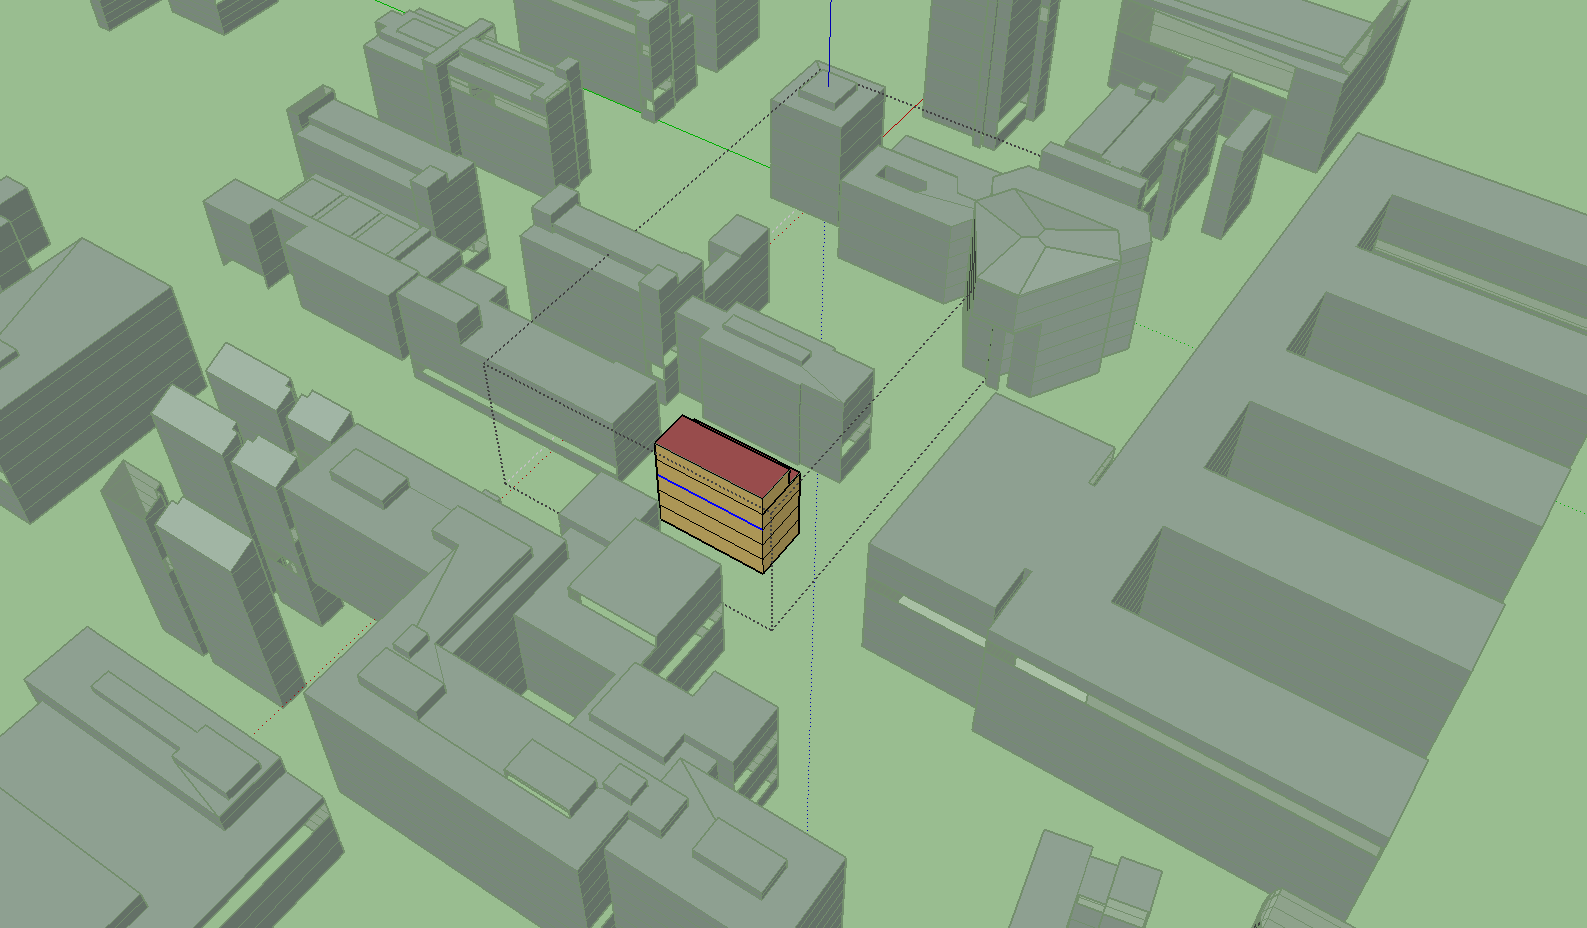
\includegraphics[scale=0.2]{figures/HPI_Campus.png}
\caption{The HPI building modeled with OpenStudio for Sketchup.}
\label{fig:HPIcampus}
\end{figure}

% \begin{figure}[H]
% \centering
% \includegraphics[scale=0.2]{figures/campuscitysim}
% \caption{Campus modeled in CitySim}
% \label{fig:campuscitysim}
% \end{figure}

\subsection{Measured data collection and calibration}

Energy data from the HPI building was collected and analyzed in the context of the simplified calibration procedures. The measured datasets are screened and aggregated into typical usage profiles to be used for the lighting, plug-loads, and HVAC equipment availability schedules and power densities. Figure \ref{fig:hpi_elec_profiles} illustrates the aggregation examples of electrical energy for the HPI building. This profile was created through a filtering and clustering process known as \emph{DayFilter} \cite{Miller:2015kr}. This profile is used to set the availability schedules as inputs into the EnergyPlus simulation to emulate the way occupants inhabit the building and how the building management system (BMS) controls the lighting and HVAC systems. This approach is compared to the practice of interviews and site visits to determine such input parameters.

\begin{figure}[H]
\centering
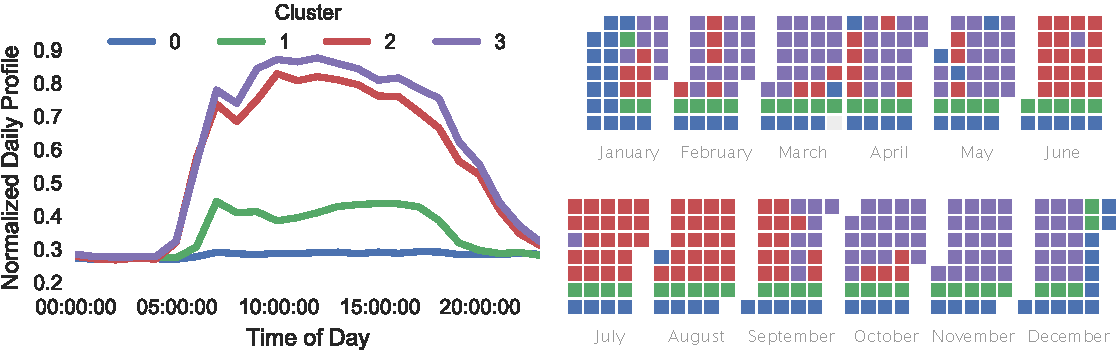
\includegraphics[scale=0.6]{figures/HPI_combinedclusterandcal_4}
\caption{HPI Electrical Energy Typical Profiles}
\label{fig:hpi_elec_profiles}
\end{figure}

The measured and simulated data from both the co-simulation and EnergyPlus solo simulations is shown in Figure \ref{fig:hpi_measvssim}.

\begin{figure}[H]
\centering
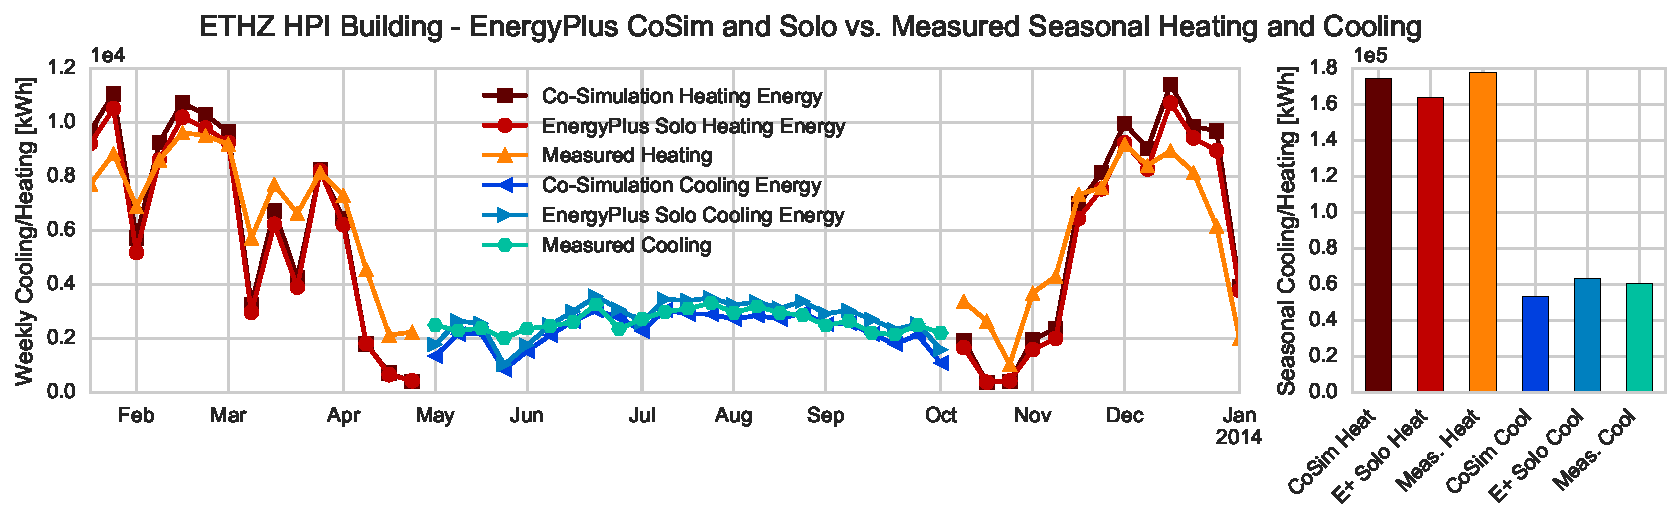
\includegraphics[scale=0.55]{figures/HPI_MeasvsSim}
\caption{HPI Measured vs. Co-Simulation and EnergyPlus Solo for Heating and Cooling Seasons}
\label{fig:hpi_measvssim}
\end{figure}

\subsection{EnergyPlus co-simulation results}

\begin{figure}[H]
\centering
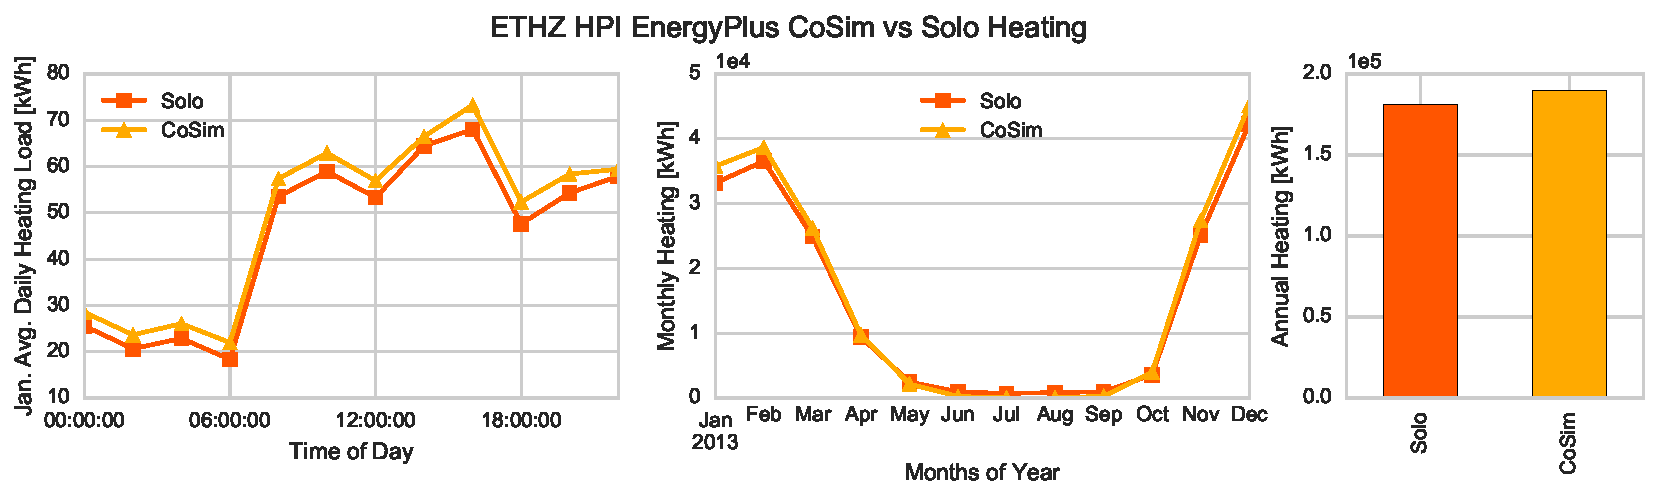
\includegraphics[scale=0.55]{figures/HPI_EnergyPlus_Heating}
\caption{HPI Co-Simulation vs. EnergyPlus Solo for Heating}
\label{fig:hpi_energyplusheating}
\end{figure}

\begin{figure}[H]
\centering
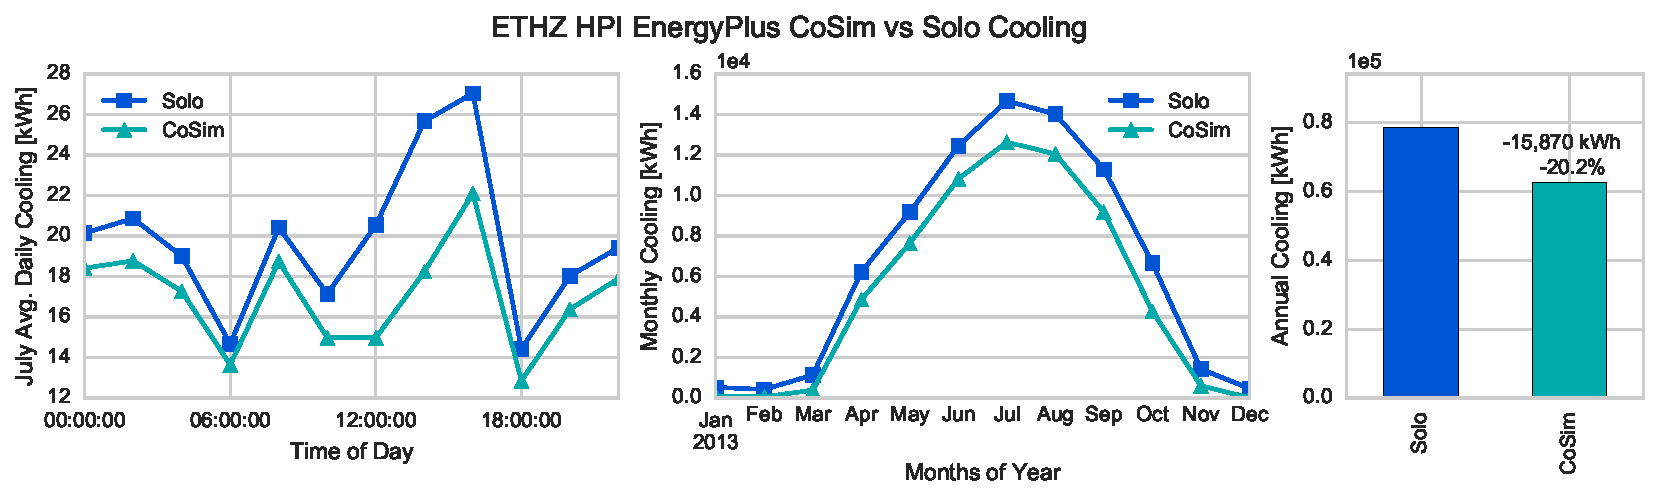
\includegraphics[scale=0.55]{figures/HPI_EnergyPlus_Cooling}
\caption{HPI Co-Simulation vs. EnergyPlus Solo for Cooling}
\label{fig:hpi_energypluscooling}
\end{figure}

% \ref{fig:hpz_profiles}-\ref{fig:hit_profiles}

% \begin{figure}
% \centering
% 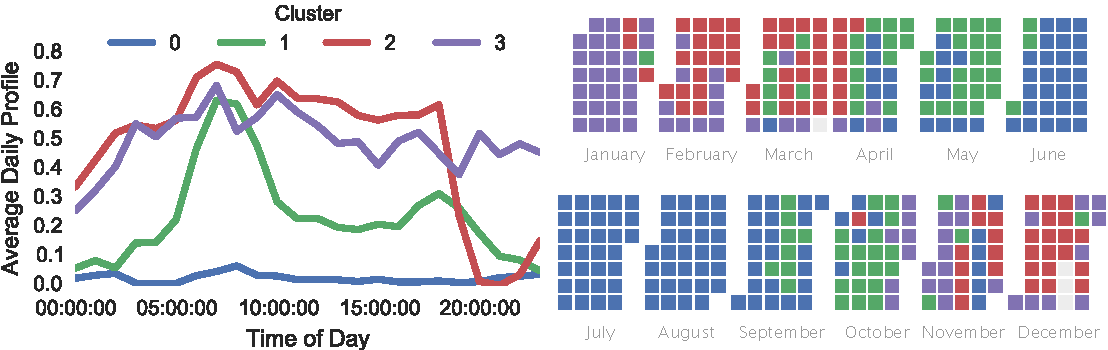
\includegraphics[scale=0.45]{figures/HPZ_combinedclusterandcal_4}
% \caption{HPZ Heating Energy Typical Profiles}
% \label{fig:hpz_profiles}
% \end{figure}

% \begin{figure}
% \centering
% 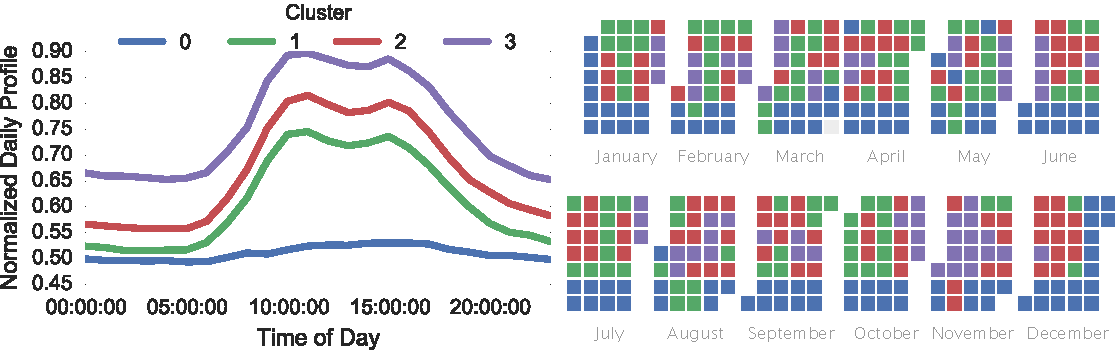
\includegraphics[scale=0.45]{figures/HPK_combinedclusterandcal_4}
% \caption{HPK Electrical Energy Typical Profiles}
% \label{fig:hpk_profiles}
% \end{figure}


% \begin{figure}
% \centering
% 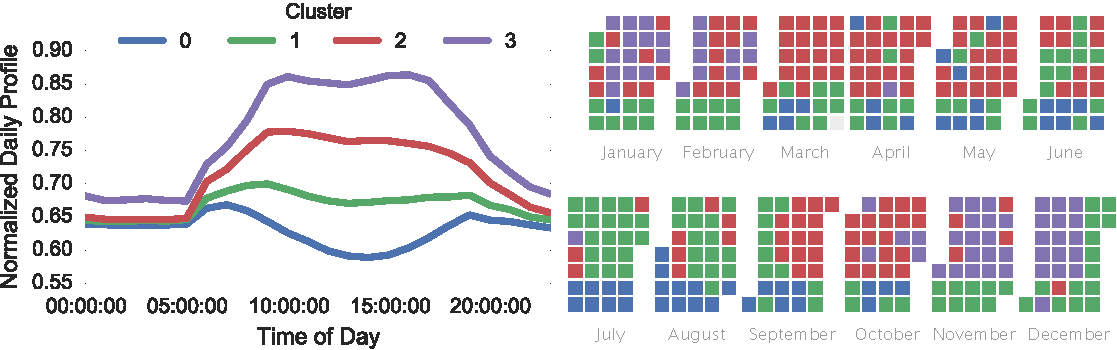
\includegraphics[scale=0.45]{figures/HIT_combinedclusterandcal_4}
% \caption{HIT Electrical Energy Typical Profiles}
% \label{fig:hit_profiles}
% \end{figure}

\subsection{Campus case study 2: EPFL Quartier Nord}
Quartier Nord is a whole new quarter of the École Polytechnique Fédérale de Lausanne (EPFL) campus located at its northwest corner. This complex includes a Convention Centre with an auditorium with a maximum capacity of 3000 (seated) people, housing for 516 students, retail and service areas and a hotel. As a public space, this ensemble is organized around a main plaza (see Figure \ref{fig:quartier_nord_1}).

\begin{figure}[H]
\centering
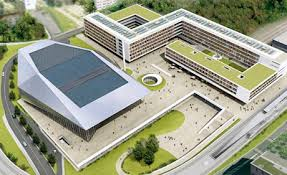
\includegraphics[]{figures/quartier_nord_1}
\caption{The Quartier Nord at EPFL in Lausanne}
\label{fig:quartier_nord_1}
\end{figure}

With a particularly strong visual and formal identity, the SwissTech Convention Centre (STCC) is clearly the key protagonist. Applied with important functions for the region, the building has definitely become the new landmark. Designed as a Minergie building, it includes modern energy conversion technologies to reduce its energy consumption. The focus of the co-simulation is realised on the STCC, simulated with the nearby buidings for housing, retail and service areas.

\subsection{Model development}
The information required in the simulation mainly comprises three parts: physical, geometrical and operational data. The geometry information including the building’s shape, dimension, structure and materials was obtained from the Real Estate and Infrastructure Department of École Polytechnique Fédérale de Lausanne (EPFL), which was responsible for carrying out the project from call to tender to construction. However, since the documents provided were full of details but also conflicting with what has been installed as compared to the documents before construction, the task to realise a precise model of the buildings itself is rather tedious. Besides, it is even more challenging to get the operational data (daily occupancy, lighting and electrical equipment usage level and ventilation rate) as the building has only recently been set in operation mode and as engineers and technicians have been working on improving the controls. Therefore, due to unreliable monitoring data, the calibration step of the model has been unfortunately abandoned.\\

Considering the lack of detailed information about the building, a so-called detailed reference case was modeled with EnergyPlus \citep{Mauree:2015} in which regulation standards applied in the design phase from the SIA norms were used to complete the missing information (see Figure \ref{fig:model_yang}).

\begin{figure}[H]
\centering
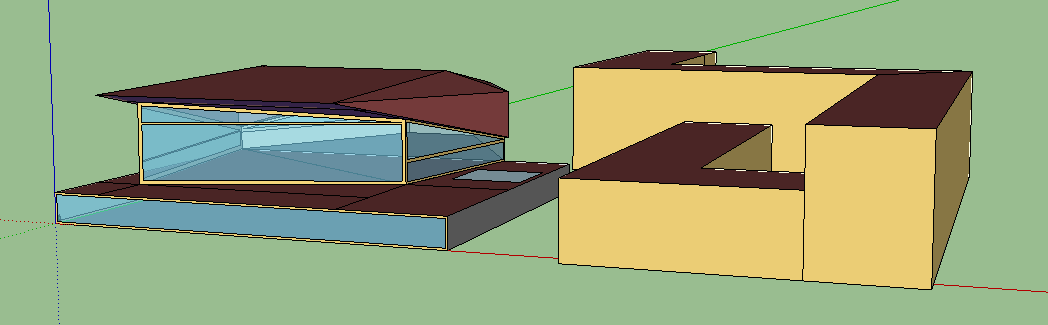
\includegraphics[width=\textwidth]{figures/model_yang}
\caption{The Quartier Nord modeled with OpenStudio for Sketchup. The STCC on the left is the main focus of the study and represented by two thermal zones.}
\label{fig:model_yang}
\end{figure}

The corresponding CitySim model was created by exporting a DXF file from EnergyPlus, and importing it into the Graphical User Interface of CitySim. Physical caracteristics of the building were added to complete the CitySim model. Finally, the same script as described in Section \ref{Methodology} was used to export the model from CitySim to EnergyPlus, giving a simplified EnergyPlus model.\\

% As a summary, three models are compared: a detailed EnergyPlus model, a simplified CitySim model and a simplified EnergyPlus model. In addition to what a coupled simplified CitySim and EnergyPlus model is realised and its results analysed with respect to the other three models. 

% \section{Results}
% {\color{red}Here we show all of the data of the comparison between the simulation outputs and the measured data from the campus}

% \section{Results}
\subsection{Comparison of EnergyPlus and CitySim}

\begin{figure}[H]
\centering
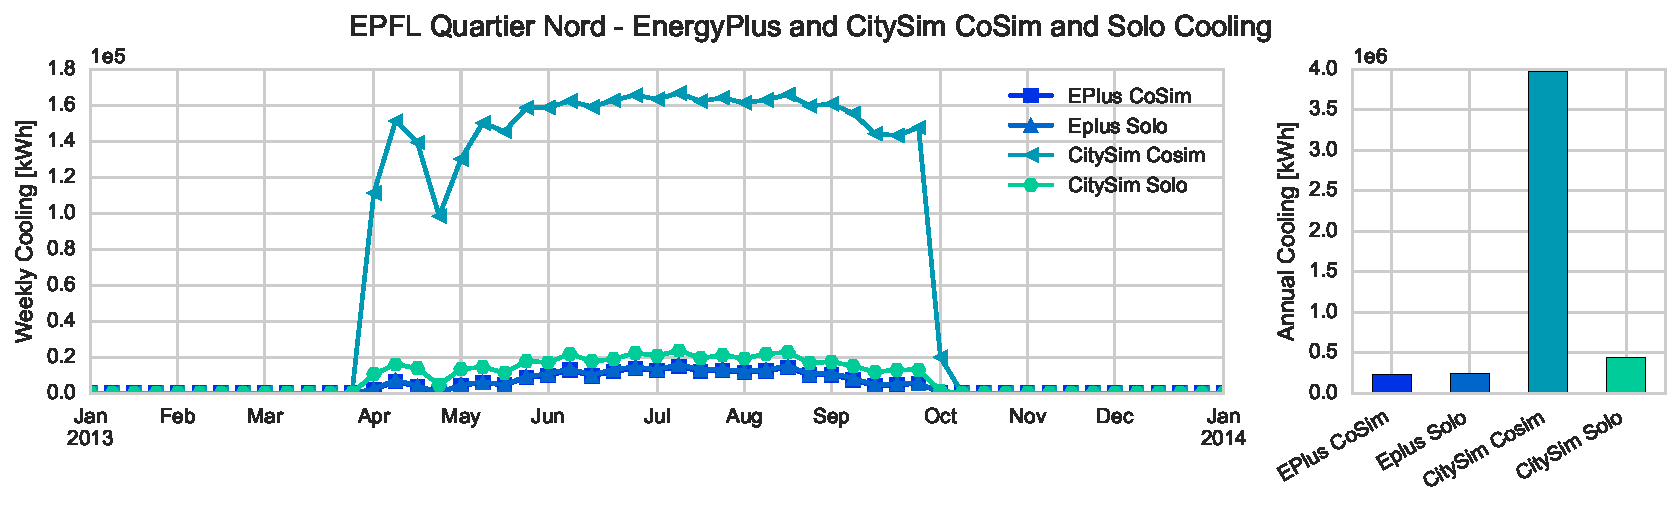
\includegraphics[scale=0.55]{figures/QN_Cooling}
\caption{Quartier Nord CitySim vs. EnergyPlus Solo for Cooling}
\label{fig:qn_eplusvscitysim_cooling}
\end{figure}

\begin{figure}[H]
\centering
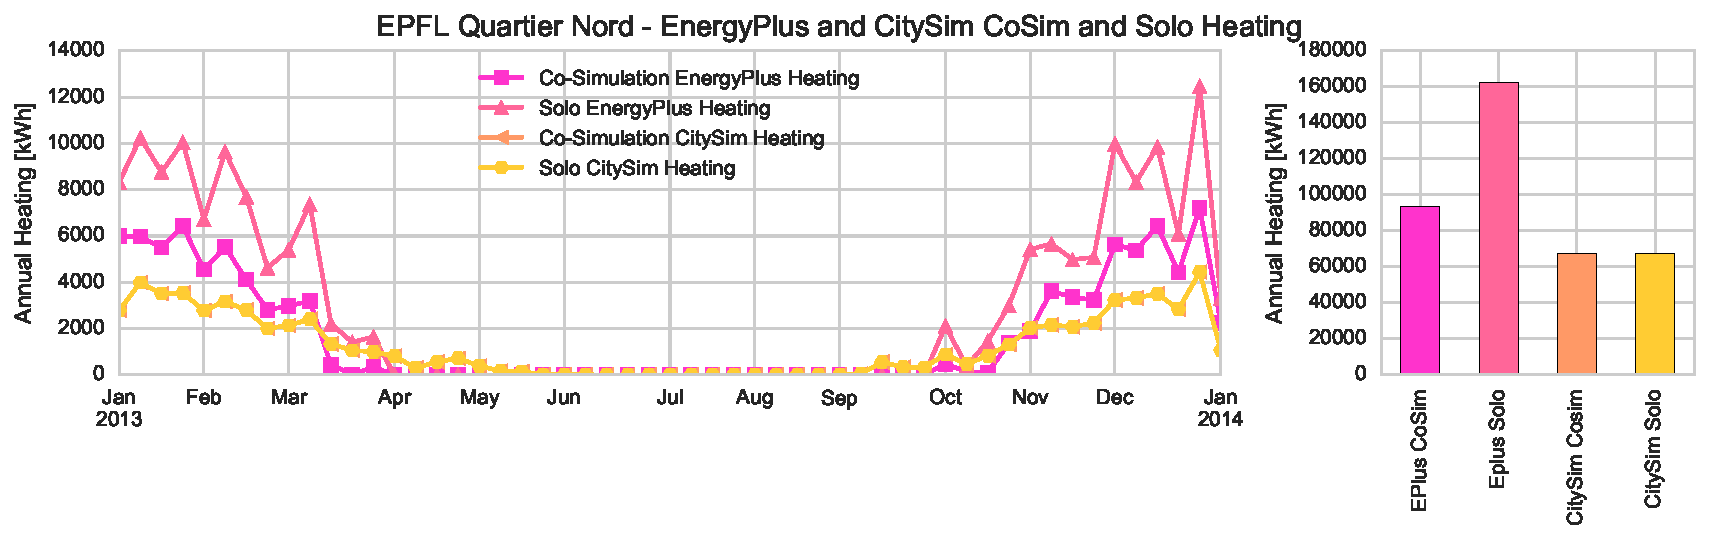
\includegraphics[scale=0.55]{figures/QN_Heating.pdf}
\caption{Quartier Nord CitySim vs. EnergyPlus Solo for Heating}
\label{fig:qn_eplusvscitysim_heating}
\end{figure}

\subsection{EnergyPlus Co-simulation results}

\begin{figure}[H]
\centering
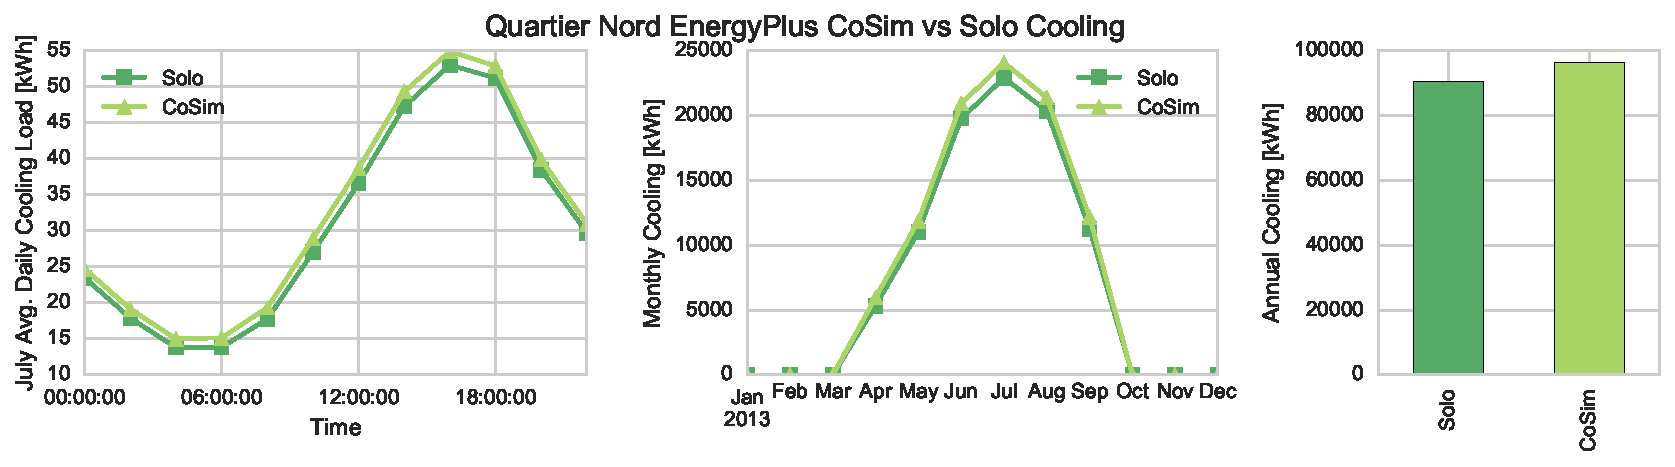
\includegraphics[scale=0.55]{figures/QN_EnergyPlus_Cooling}
\caption{Quartier Nord EnergyPlus Co-Simulation vs. Solo for Cooling}
\label{fig:qn_eplus_cosimvssolo_cooling}
\end{figure}

\begin{figure}[H]
\centering
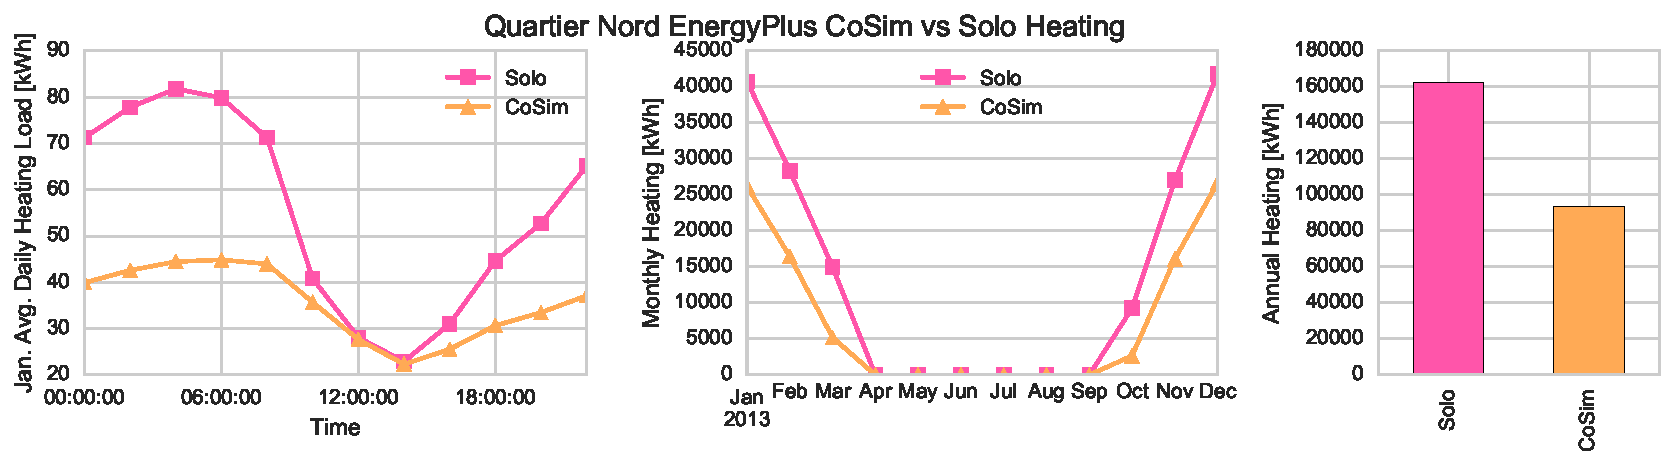
\includegraphics[scale=0.55]{figures/QN_EnergyPlus_Heating}
\caption{Quartier Nord EnergyPlus Co-Simulation vs. Solo for Heating}
\label{fig:qn_eplus_cosimvssolo_heating}
\end{figure}

\subsection{CitySim Co-simulation results}

\begin{figure}[H]
\centering
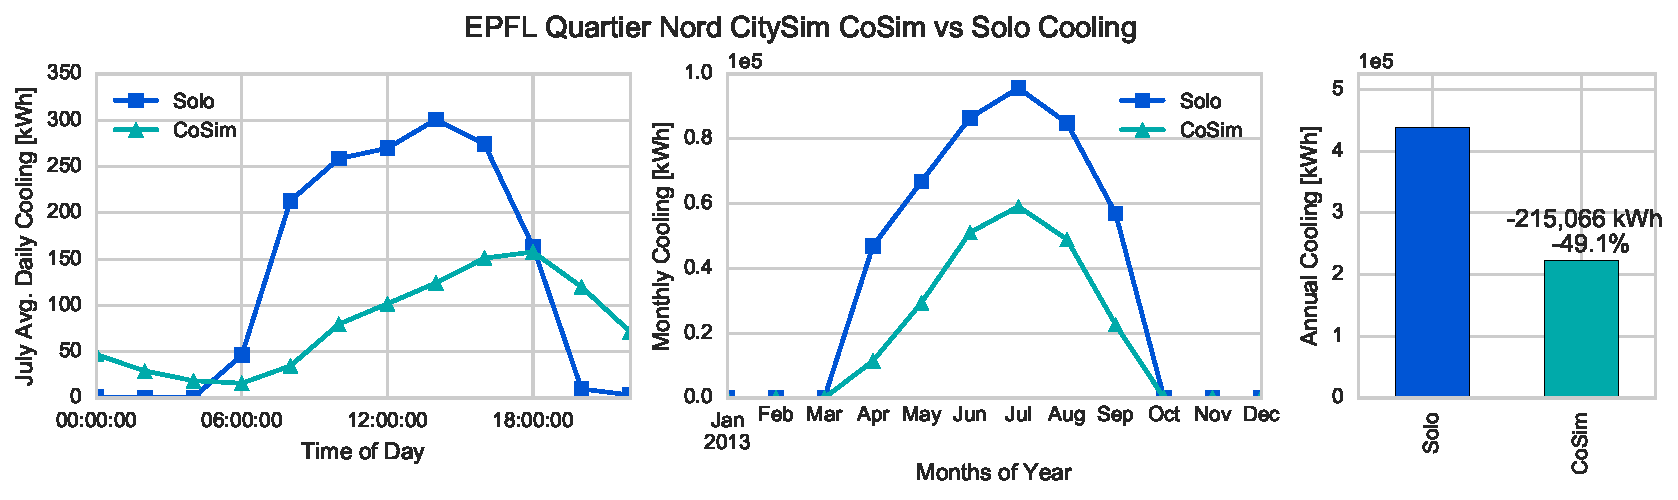
\includegraphics[scale=0.55]{figures/QN_CitySim_Cooling}
\caption{Quartier Nord CitySim Co-Simulation vs. Solo for Cooling}
\label{fig:qn_citysim_cosimvssolo_cooling}
\end{figure}

\begin{figure}[H]
\centering
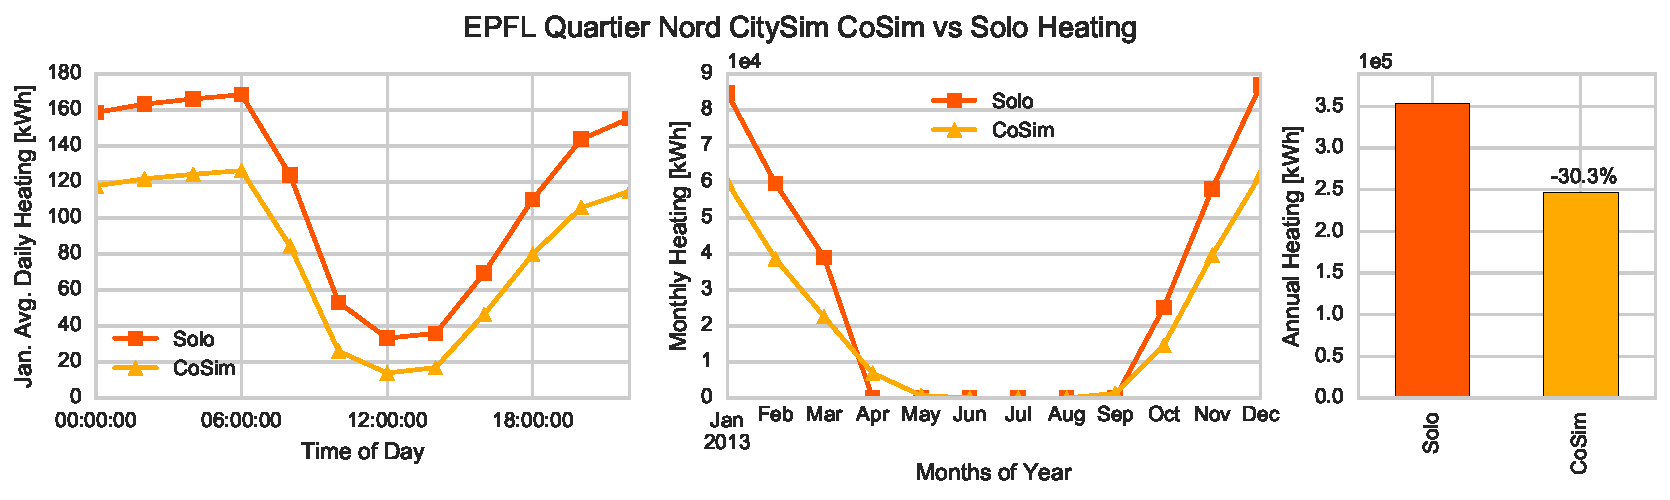
\includegraphics[scale=0.55]{figures/QN_CitySim_Heating}
\caption{Quartier Nord CitySim Co-Simulation vs. Solo for Heating}
\label{fig:qn_citysim_cosimvssolo_heating}
\end{figure}


\section{Conclusion}

\subsection{Acknowledgements}

The authors would like to acknowledge the ETH Z\"urich Campus Facilities Department and the EPFL Real Estate and Infrastructure Department. This research was funded by the Competence Center in Energy and Mobility (CCEM) under the UMEM project.

\bibliographystyle{tBPS}
\bibliography{UMEM_CoSim}


\end{document}
